\documentclass[11pt]{article}

\usepackage[a4paper]{geometry}
\geometry{left=2.0cm,right=2.0cm,top=2.5cm,bottom=2.5cm}

\usepackage{ctex} % 支持中文的LaTeX宏包
\usepackage{amsmath,amsfonts,graphicx,subfigure,amssymb,bm,amsthm,mathrsfs,mathtools,breqn} % 数学公式和符号的宏包集合
\usepackage{algorithm,algorithmicx} % 算法和伪代码的宏包
\usepackage[noend]{algpseudocode} % 算法和伪代码的宏包
\usepackage{fancyhdr} % 自定义页眉页脚的宏包
\usepackage[framemethod=TikZ]{mdframed} % 创建带边框的框架的宏包
\usepackage{fontspec} % 字体设置的宏包
\usepackage{adjustbox} % 调整盒子大小的宏包
\usepackage{fontsize} % 设置字体大小的宏包
\usepackage{tikz} % 绘制图形和使用颜色的宏包
\usetikzlibrary{arrows.meta} % TikZ箭头库
\usepackage{float} % 支持[H]浮动体位置参数
\usepackage{multicol} % 多栏排版的宏包
\usepackage{multirow} % 表格中合并单元格的宏包
\usepackage{pdfpages} % 插入PDF文件的宏包
\RequirePackage{listings} % 在文档中插入源代码的宏包
\usepackage{wrapfig} % 文字绕排图片的宏包
\usepackage{bigstrut,multirow,rotating} % 支持在表格中使用特殊命令的宏包
\usepackage{booktabs} % 创建美观的表格的宏包
\usepackage{circuitikz} % 绘制电路图的宏包
\usepackage{hyperref} % 创建超链接的宏包
\usepackage[inline]{enumitem} % 自定义列表格式的宏包，支持行内列表

\definecolor{dkgreen}{rgb}{0,0.6,0}
\definecolor{gray}{rgb}{0.5,0.5,0.5}
\definecolor{mauve}{rgb}{0.58,0,0.82}
\lstset{
  frame=tb,
  aboveskip=3mm,
  belowskip=3mm,
  showstringspaces=false,
  columns=flexible,
  framerule=1pt,
  rulecolor=\color{gray!35},
  backgroundcolor=\color{gray!5},
  basicstyle={\small\ttfamily},
  numbers=none,
  numberstyle=\tiny\color{gray},
  keywordstyle=\color{blue},
  commentstyle=\color{dkgreen},
  stringstyle=\color{mauve},
  breaklines=true,
  breakatwhitespace=true,
  tabsize=3,
}


\usepackage[capitalize]{cleveref}
\Crefname{section}{Section}{Sections}
\Crefname{table}{Table}{Tables}
\crefname{table}{Table.}{Tabs.}

\setmainfont{Palatino Linotype}
\setCJKmainfont{SimSun}[BoldFont=SimHei, ItalicFont=KaiTi]
\setCJKsansfont{SimHei}
\setCJKmonofont{FangSong}
\punctstyle{kaiming}
% 偏好的几个字体, 可以根据需要自行加入字体ttf文件并调用

% Restore standard emphasis to avoid requiring an undefined environment (kaishu).
% The original redefinition used an environment `kaishu` which is not defined
% in a default ctex setup and causes compilation errors. Use \textit for
% emphasis which works across engines.
\renewcommand{\emph}[1]{\textit{#1}}

%改这里可以修改实验报告表头的信息
\newcommand{\experiName}{激光光路}
\newcommand{\supervisor}{董国艳}
\newcommand{\name}{邓思豪}
\newcommand{\studentNum}{2023K8009909008}
\newcommand{\class}{3}
\newcommand{\group}{01}
\newcommand{\seat}{5}
\newcommand{\dateYear}{2025}
\newcommand{\dateMonth}{10}
\newcommand{\dateDay}{29}
\newcommand{\room}{西实201}
\newcommand{\others}{$\square$}


\begin{document}



\begin{center}
    \LARGE \bf 《\, 基\, 础\, 物\, 理\, 实\, 验\, 》\, 实\, 验\, 报\, 告
\end{center}

\begin{center}
    \noindent \emph{实验名称}\underline{\makebox[25em][c]{\experiName}}
    \emph{指导教师}\underline{\makebox[8em][c]{\supervisor}}\\
    \emph{姓名}\underline{\makebox[6em][c]{\name}} 
    % 如果名字比较长, 可以修改box的长度"6em"
    \emph{学号}\underline{\makebox[10em][c]{\studentNum}}
    \emph{分班分组及座号} \underline{\makebox[5em][c]{\class \ -\ \group \ -\ \seat }\emph{号}} （\emph{例}:\, 1\,-\,04\,-\,5\emph{号}）\\
    \emph{实验日期} \underline{\makebox[3em][c]{\dateYear}}\emph{年}
    \underline{\makebox[2em][c]{\dateMonth}}\emph{月}
    \underline{\makebox[2em][c]{\dateDay}}\emph{日}
    \emph{实验地点}\underline{{\makebox[6em][c]\room}}
    \emph{调课/补课} \underline{\makebox[3em][c]{\others\ 是}}
    \emph{成绩评定} \underline{\hspace{5em}}
    {\noindent}
    \rule[8pt]{17cm}{0.2em}
\end{center}

\section{实验目的}本实验围绕激光的原理、传输、干涉、偏振及光纤耦合与参数测量展开，具体内容如下：

\begin{enumerate}
    \item \textbf{激光产生原理与传输接收特性的系统学习}：深入剖析激光受激辐射、粒子数反转等基本产生机制，全面掌握激光在传播过程中的相干性、方向性、单色性等核心特性，同时理解激光接收系统的架构与性能要求。
    \item \textbf{激光传输、扩束实验现象的观测与分析}：构建激光传输光路，观测激光在自由空间的准直传输行为；通过扩束装置研究光束口径与发散角的调控规律，对不同传输场景下的实验现象进行记录与物理机制阐释。
    \item \textbf{基于马赫—曾德干涉仪的激光光路调节方法掌握}：搭建马赫—曾德干涉仪实验系统，学习分束、合束光路的准直与共路调节技术，掌握激光干涉光路中光程差与相干条纹的调控方法，理解光路调节精度对干涉效果的影响。
    \item \textbf{激光偏振态的检偏器检验技术学习}：利用检偏器搭建偏振检测光路，探究线偏振、圆偏振等不同偏振态的检验原理与操作流程，分析偏振态与检偏器角度的定量关系，深化对激光偏振特性的认知。
    \item \textbf{空间光耦合进光纤的调整方法学习与耦合效率提升探究}：理解空间激光与光纤耦合的基本原理，掌握耦合光路的对准、聚焦等调整技巧；分析光斑模式、对准精度、聚焦参数等对耦合效率的影响，并探索提升耦合效率的技术路径。
    \item \textbf{光纤数值孔径测量方法的掌握}：明确数值孔径作为光纤关键光学参数的物理内涵，搭建数值孔径测量实验装置，掌握远场法或近场法等测量技术的操作规范，实现对光纤数值孔径的精确测量与结果分析。
\end{enumerate}

\section{实验器材清单}
以下为本次光学实验所需的器材及其规格、功能说明：
\begin{itemize}
    \item 光学平板：尺寸为\(60\mathrm{cm} \times 60\mathrm{cm}\)，作为搭建光学实验光路的基础承载平台，为各光学元件的排布提供稳定支撑。
    \item 氦氖激光器：一台，输出激光波长为\(632.8\mathrm{nm}\)，具备优异的单色性与相干性，为实验提供高品质的激光光源。
    \item 增强铝反射镜：四套，采用增强铝镀膜工艺，具有高反射率，用于灵活改变激光光路的传播方向，实现光路的空间布局调整。
    \item 无偏振分光棱镜：两个，可将入射光按特定比例分为两束光，且不引入偏振态差异，是实现光的分束与干涉实验的关键元件。
    \item 透镜组：一套，包含焦距分别为\(-30\mathrm{mm}\)（凹透镜）和\(150\mathrm{mm}\)（凸透镜）的透镜，放大倍率为\(1:5\)，用于完成光束的会聚、发散、成像等光学变换操作。
    \item 起偏器与检偏器：各一个，配合使用可产生线偏振光并对光的偏振态进行检测，是探究光的偏振特性实验的核心器材。
    \item 光电池（功率计）：一个，能够对激光的光功率进行定量测量，实现光强的精确检测与分析。
    \item 半导体激光器：一台，输出波长为\(650\mathrm{nm}\)，可作为辅助光源或用于特定波长的光学现象研究。
    \item 三维加旋转调整架：一套，可对光学元件进行三维空间位置及旋转角度的精细调节，满足光路对准的多自由度调整需求。
    \item 五维调整架：一套，具备五个维度的精密调节功能，适用于复杂光路中光学元件的高精度对准操作。
    \item 光纤支架：一个，用于对光纤进行稳定固定，确保光纤在光路中的空间位置稳定性。
    \item 光纤红光笔：一个，通过发射红光实现光纤通路的快速导通检测，为光纤光路的搭建与调试提供辅助。
    \item 光纤：单模光纤、多模光纤各一条，可用于开展光纤传输特性、模式分布等光纤光学相关实验研究。
    \item 显示屏：一个，用于实时显示实验数据、光路成像结果等信息，便于实验观测与分析。
    \item 直尺：一把，刻度单位为\(\mathrm{cm}\)，用于光路中距离的测量与空间尺度的标定。
    \item 激光防护镜：一套，为实验人员提供眼部防护，有效避免激光对眼睛造成损伤，保障实验安全。
\end{itemize}

\section{实验原理}
\subsection{马赫-曾德尔（M-Z）干涉仪的工作原理}

马赫-曾德尔（Mach-Zehnder, M-Z）干涉仪是一种基于**分振幅双光束干涉**的经典光学装置，其核心原理是通过对相干光的“分束-光程差引入-合束”过程，利用相位差的空间分布产生可观测的干涉条纹，从而实现对光场相位、介质光学参数等物理量的高精度探测。


\subsubsection{电场与光强的理论推导}
由同一激光光源发出的**相干光**，经**无偏振分光棱镜**分为光强比为$1:1$、偏振态一致的两束光，分别定义为**信号光**和**参考光**。两束光沿不同路径传输（即经历不同**光程**）后重新合束，由于合束区域内不同位置处两束光的**相位差**存在差异，最终在探测平面形成干涉条纹。

假设合束光斑某一位置处，两束光的**复电场矢量**可表示为：
\begin{align}
E_1(t) &= E_0 e^{-i\omega t + i\phi_1(t)} \\
E_2(t) &= E_0 e^{-i\omega t + i\phi_2(t)}
\end{align}
其中，$E_0$为电场振幅，$\omega$为光的角频率，$\phi_1(t)$和$\phi_2(t)$分别为信号光与参考光的瞬时相位。

光强是电场强度的**时间平均值**（对光的振荡周期积分），根据光强定义$I = \langle E \cdot E^* \rangle$（$E^*$为电场的复共轭），对两束光的合场强进行时间平均后，可得该位置的光强为：
\begin{equation}
I(t) = I_1 + I_2 + 2\sqrt{I_1 I_2} \cos\Delta\phi
\end{equation}
其中，$I_1 = I_2 = \langle |E_0|^2 \rangle$（因分束光强比为$1:1$），$\Delta\phi = \phi_1(t) - \phi_2(t)$为两干涉臂的**相位差**。式中第三项为**干涉项**，其随$\Delta\phi$的周期性变化（$0 \sim 2\pi$）直接对应干涉条纹的“明-暗-明”交替分布。


\subsubsection{典型光路结构}
M--Z 干涉仪的典型光路如图\ref{fig:MZ_optics}所示，主要由 \textbf{He--Ne 激光器}、反射镜、准直扩束系统（平凸透镜）、无偏振分光棱镜等光学元件构成。
\begin{itemize}
  \item 激光经平凸透镜准直扩束后，由第一块分光棱镜分为两路光束；
  \item 两路光束分别经反射镜改变传播方向，其中一路可引入待测信号（如介质折射率变化、光程扰动等），另一路作为参考光保持光程稳定；
  \item 最终两路光由第二块分光棱镜合束，在探测区域（或成像平面）形成\emph{等厚/等倾干涉条纹}（见干涉条纹示意）。
\end{itemize}

\begin{figure}[htbp]
  \centering
  \subfigure[马赫--曾德尔干涉仪光路结构示意图\label{fig:MZ_optics_path}]{%
    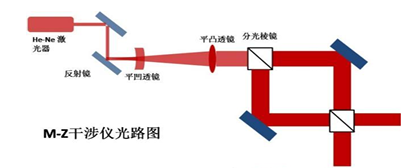
\includegraphics[width=0.60\textwidth]{MZ_optical_path.png}%
  }\hfill
  \subfigure[干涉条纹示意图\label{fig:MZ_optics_fringes}]{%
    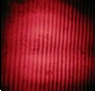
\includegraphics[width=0.30\textwidth]{MZ_fringes.png}%
  }
  \caption{马赫--曾德尔（Mach--Zehnder）干涉仪原理图及干涉条纹示意}
  \label{fig:MZ_optics}
\end{figure}

\subsection{马吕斯定律与偏振光的起偏--检偏原理}

偏振现象是横波的固有特性。利用偏振片实现的“起偏—检偏”过程是偏振态调控与探测的基本手段，\textbf{马吕斯定律（Malus's law）}定量描述了线偏振光通过检偏器后的透射光强度。

\subsubsection{偏振片的结构与偏振器的分类}
偏振片通常由具有吸收或双折射性质的分子或薄膜制成，其分子取向导致对特定振动方向的光允许通过，而对正交方向吸收或阻挡。根据用途，偏振片可分为：
\begin{itemize}
  \item \textbf{起偏器}：将自然光（非偏振光）转换为近似线偏振光的器件；
  \item \textbf{检偏器}：用于分析线偏振光的偏振方向并测量透射光强的器件。
\end{itemize}

\subsubsection{马吕斯定律的理论推导}\label{subsub:malus}
设入射线偏振光的电场振幅为 $E_0$，若起偏器与检偏器的偏振轴夹角为 $\phi$，则沿检偏器光轴的电场分量为：
\begin{equation}\label{eq:malus_E}
  E = E_0\cos\phi
\end{equation}
光强与电场振幅的平方成正比，若透过起偏器的光强为 $I_0$（即 $I_0\propto E_0^2$），则透过检偏器的光强为：
\begin{equation}\label{eq:malus}
  I = I_0\cos^2\phi
\end{equation}
式\eqref{eq:malus}即为马吕斯定律，描述了透射光强与偏振轴夹角之间的关系。

\subsubsection{极端情况与应用}
由式\eqref{eq:malus}可得以下极端情况：
\begin{itemize}
  \item 当 $\phi=0^\circ$（两偏振轴平行）时，$\cos^2\phi=1$，故 $I=I_0$，透射光强达最大；
  \item 当 $\phi=90^\circ$（两偏振轴正交）时，$\cos^2\phi=0$，故 $I=0$，发生完全消光；
  \item 当 $0^\circ<\phi<90^\circ$ 时，透射光强介于 $0$ 与 $I_0$ 之间，并随 $\cos^2\phi$ 变化。
\end{itemize}

上述特性在偏振检测、偏振成像与显示技术（例如液晶显示）中有广泛应用：利用正交偏振的消光可实现偏振态的高精度检测与校准。

\begin{figure}[htbp]
  \centering
  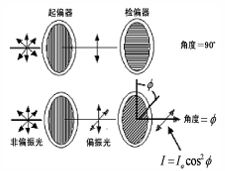
\includegraphics[width=0.6\textwidth]{polarization_detection.png}
  \caption{偏振光检测示意图：起偏器与检偏器的偏振轴夹角 $\phi$ 对透射光强的影响（遵循 $I=I_0\cos^2\phi$）。}
  \label{fig:polarization_detection}
\end{figure}

图\ref{fig:polarization_detection}展示了偏振轴夹角 $\phi$ 对透射光强的影响：$\phi=90^\circ$ 时透射光消失，其余角度则按式\eqref{eq:malus}变化。


\subsection{光纤耦合原理、分类与数值孔径}

光纤是光通信与光传感领域的核心传输介质，其工作基于\textbf{全内反射导光机制}，而光纤耦合技术是实现光信号在光纤与其他光器件间高效传输的关键。以下从结构、分类、数值孔径及耦合技术四个维度展开分析。


\subsubsection{光纤的结构与导光机制}
光纤由\textbf{纤芯}、\textbf{包层}和\textbf{保护套}三层构成（如图\ref{fig:fiber_structure}所示）：
\begin{itemize}
  \item \textbf{纤芯}：折射率 $n_1$ 较高，是光信号传输的核心区域；
  \item \textbf{包层}：折射率 $n_2 < n_1$，与纤芯形成全内反射的边界条件；
  \item \textbf{保护套}：提供机械防护，承受冲击并保护光纤。
\end{itemize}

当光在纤芯--包层界面的入射角大于\textbf{临界角}时，发生\textbf{全内反射}，使光被"闭锁"在纤芯内向前传播。从波动光学角度，麦克斯韦方程在光纤边界下的解表现为"传输模式"：仅支持一种模式的为单模光纤，支持多种模式的为多模光纤。

\begin{figure}[htbp]
  \centering
  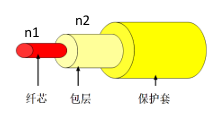
\includegraphics[width=0.5\textwidth]{fiber_structure.png} % 替换为图3实际文件名
  \caption{光纤结构示意图（纤芯、包层、保护套）}
  \label{fig:fiber_structure}
\end{figure}


\subsubsection{光纤的分类体系}
光纤可从传输模式、材料成分、折射率分布三个维度分类：

\paragraph{按传输模式分类}
\begin{itemize}
  \item \textbf{单模光纤}：仅传输\textbf{基模}，纤芯直径通常 $<10\ \mu\text{m}$。具有带宽高、衰减低、色散小的优点，适用于长距离高速通信（如干线网、城域网）。
  \item \textbf{多模光纤}：可传输多个模式，纤芯直径通常 $\geq50\ \mu\text{m}$。带宽低、衰减大但成本低、易耦合，适用于短距离场景（如局域网、数据中心内部）。
\end{itemize}


\paragraph{按材料成分分类}
\begin{itemize}
  \item \textbf{石英光纤}：以二氧化硅为主要原料，物理化学稳定性优异、衰减小，是通信领域的主流类型。
  \item \textbf{塑料光纤}：以聚合物为芯材，柔软易弯曲、成本低，但衰减大、带宽有限，适用于短距离场景（如家庭网络、汽车内部通信）。
\end{itemize}


\paragraph{按折射率分布分类}
\begin{itemize}
  \item \textbf{阶跃折射率光纤}：纤芯与包层折射率\textbf{突变}，模式色散大，多用于早期多模系统。
  \item \textbf{渐变折射率光纤}：纤芯折射率从中心向外\textbf{渐变降低}，可抑制模式色散，适用于现代多模系统。
\end{itemize}


\subsubsection{数值孔径（NA）的定义与应用}
数值孔径是描述光纤\textbf{集光能力}的关键参数，定义为入射光最大接收角的正弦值，公式为：
\begin{equation}\label{eq:NA}
NA = \sin\theta_n = \sqrt{n_1^2 - n_2^2}
\end{equation}
其中 $\theta_n$ 为数值孔径角，$n_1$、$n_2$ 分别为纤芯、包层折射率。

\paragraph{物理意义与特性}
\begin{itemize}
  \item $NA$ 越大，光纤集光能力越强，耦合效率越高，但模式色散也越大（限制传输容量）。例如单模光纤典型 $NA\approx0.13$，对应接收角约 $7.5^\circ$。
  \item 可通过光斑区分单/多模光纤：单模光纤光斑为"中心强、边缘弱"的圆斑；多模光纤为多模式叠加的"梅花状"光斑（如图\ref{fig:fiber_mode}所示）。
\end{itemize}

\begin{figure}[htbp]
  \centering
  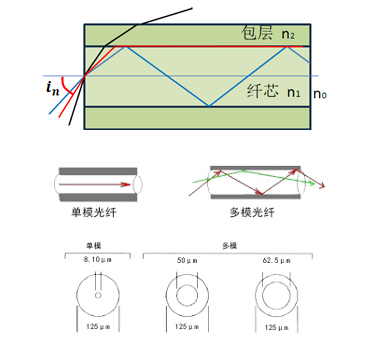
\includegraphics[width=0.6\textwidth]{fiber_mode.png} % 替换为图4实际文件名
  \caption{光纤导光原理与单/多模光纤光斑、芯径对比}
  \label{fig:fiber_mode}
\end{figure}

\paragraph{数值孔径的测量方法}
\begin{itemize}
  \item \textbf{远场法}：测量远场辐射图中光强降至中心最大值 $\frac{1}{e^2}$ 处的半角正弦值，即为 $NA$。
  \item \textbf{计算法}：直接通过 $n_1$、$n_2$ 代入公式 $NA = \sqrt{n_1^2 - n_2^2}$ 计算。
\end{itemize}


\subsubsection{光纤耦合技术：方式、效率与优化}
光纤耦合是将光高效导入/导出光纤的过程，核心目标是\textbf{最大化耦合效率、最小化损耗}。

\paragraph{耦合方式分类}
\begin{itemize}
  \item \textbf{直接耦合}：光纤直接对准光源，结构简单但耦合效率极低（通常 $<10\%$）。
  \item \textbf{间接耦合（透镜耦合）}：通过透镜系统对光源光整形，使其与光纤的 $NA$、芯径匹配，效率可提升至数十甚至90\%以上（如图\ref{fig:lens_coupling}所示）。
\end{itemize}

\begin{figure}[htbp]
  \centering
  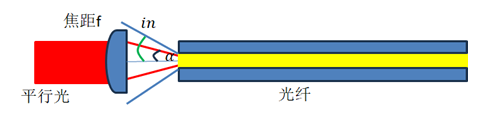
\includegraphics[width=0.6\textwidth]{lens_coupling.png} % 替换为图6实际文件名
  \caption{透镜耦合示意图（平行光经透镜聚焦入光纤）}
  \label{fig:lens_coupling}
\end{figure}

\paragraph{透镜耦合的优化条件}
要实现高效透镜耦合，需满足以下条件：
\begin{enumerate}
  \item \textbf{光束尺寸匹配}：聚焦后光束腰半径 $<$ 光纤芯径，发散角 $<$ 数值孔径角；单模光纤还需修正球差，透镜通光孔径至少为光束直径的2倍以减少衍射损耗。
  \item \textbf{光轴对准}：光束腰斑需落在光纤端面，且入射光、透镜、光纤光轴严格同轴。
  \item \textbf{损耗抑制}：通过镀增透膜、保持端面清洁，减少反射、散射与吸收损耗。
\end{enumerate}

\paragraph{耦合效率的定义与测试}
耦合效率 $\eta$ 定义为\textbf{光纤接收的有效光功率} $P_f$ 与\textbf{光源总辐射功率} $P_s$ 的比值：
\begin{equation}\label{eq:coupling_efficiency}
\eta = \frac{P_f}{P_s} \times 100\%
\end{equation}

实验中采用"显微镜系统+功率计"测试光路（如图\ref{fig:coupling_test}所示）：He--Ne激光经反射镜、显微镜聚焦后耦合入光纤，最终由光电池或功率计测量接收功率，进而计算 $\eta$。

\begin{figure}[htbp]
  \centering
  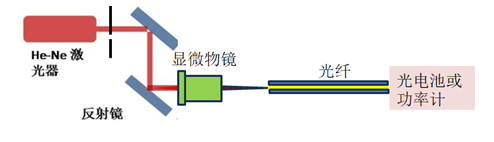
\includegraphics[width=0.7\textwidth]{coupling_test.png} % 替换为图7实际文件名
  \caption{光纤耦合效率测试光路示意图}
  \label{fig:coupling_test}
\end{figure}

\subsection{激光输出观察与基本光路的精密搭建}

光学实验中，激光光路的精准搭建是获取可靠实验结果的前提。以下从光路规划、高度标定、器件配置及准直调节四个方面，阐述规范的光路搭建方法。


\subsubsection{光路的规划与器件布局原则}
光学平台的孔线是光路规划的天然参考，需遵循以下布局规范：
\begin{itemize}
  \item \textbf{孔线对齐性}：以平台孔线为基准，初步规划反射镜、分束器等器件的空间位置，使光路沿孔线延伸，为后续精密准直提供几何约束。
  \item \textbf{功能分区性}：根据“光源-调制-传输-探测”的功能链，合理分配器件间距，既保证光程的可调控性，又预留足够的操作空间以满足调试需求。
\end{itemize}


\subsubsection{光路高度的标定方法}
光路高度的一致性是光轴共线的基础，通常以\textbf{激光器输出口中心高度}为绝对基准：
\begin{itemize}
  \item 对于反射镜、分束器等带镜面的光学元件，需通过调节架将其镜面中心高度与激光器出口高度严格对齐，确保光轴在竖直方向无偏移；
  \item 光闸的高度标定采用“激光穿孔法”：将光闸贴近激光出口，调整其高度使激光束精准穿过光闸小孔中心。光闸兼具\textbf{光强控制}与\textbf{安全防护}功能，可在调试中随时遮挡光束，保障操作安全。
\end{itemize}


\subsubsection{激光器的固定与光闸的功能配置}
\begin{itemize}
  \item \textbf{激光器的稳定化固定}：将 He--Ne 激光器沿平台孔线精准固定，开启电源后需确认激光束出射稳定、无角漂移，其细激光束作为整个光路的“种子光”，为后续光路搭建提供基准。
  \item \textbf{光闸的多功能集成}：光闸置于激光出口处，是光传输的“可控开关”——开启时允许激光通过，关闭时完全阻断光束，便于在器件调整阶段实现光的“通-断”控制，同时避免激光直射对人眼的伤害。
\end{itemize}


\subsubsection{准直光路的精密调节与专业原理}

准直是光路搭建的核心环节，需采用“迭代式远-近协同调节法”，其原理与步骤如下：

\paragraph{标靶系统构建}
将两个高度已标定的光闸 $a$ 和 $b$ 固定于规划光路上，$b$ 应在空间允许下尽可能远离 $a$，形成“近标靶-远标靶”的双标靶体系，为光轴直线性提供量化判断依据。

\paragraph{反射镜粗定位}
粗略摆放反射镜 $A$ 和 $B$，调整其位置使激光束大致同时穿过光闸 $a$ 和 $b$，随后锁定反射镜的初步位置。

\paragraph{迭代准直过程}
\begin{enumerate}
  \item \textbf{近标靶调节}：缩小光闸 $a$ 的孔径至最小，调节反射镜 $A$ 的调节螺母，使激光束精准穿过光闸 $a$ 的小孔；
  \item \textbf{远标靶调节}：放开光闸 $a$，缩小光闸 $b$ 的孔径至最小，调节反射镜 $B$ 的调节螺母，使激光束精准穿过光闸 $b$ 的小孔；
  \item \textbf{循环迭代}：重复上述步骤，因调节 $B$ 可能导致激光偏离 $a$，需再次调节 $A$ 使激光穿过 $a$，再调节 $B$ 使激光穿过 $b$。经过多个周期的迭代，最终实现激光束同时精准穿过 $a$ 和 $b$，完成光路的高精度准直。
\end{enumerate}

该过程的核心原理是 \textbf{“远调远，近调近”}：对远处的标靶 $b$，调节靠近 $b$ 的反射镜 $B$（远调远）；对近处的标靶 $a$，调节靠近 $a$ 的反射镜 $A$（近调近）。通过迭代消除光轴的偏折分量，使光沿严格的直线传输（原理如图\ref{fig:optical_collimation}所示）。

\begin{figure}[htbp]
  \centering
  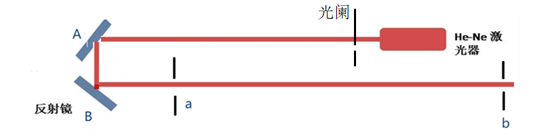
\includegraphics[width=0.6\textwidth]{optical_collimation.png} % 请替换为图8实际文件名
  \caption{光路准直原理图（反射镜A、B与光闸a、b的协同调节机制）}
  \label{fig:optical_collimation}
\end{figure}

\subsection{马赫--曾德尔（M--Z）干涉仪的搭建与干涉条纹精密观测}

马赫--曾德尔干涉仪的干涉效果依赖于相干光场的质量与光路匹配精度。下面从扩束、分束、合束与条纹观测四个环节，介绍规范的搭建与分析方法。


\subsubsection{扩束系统的原理与精密搭建}
激光束腰尺寸极小，相干面积有限。为获得\textbf{高对比度、大视场的干涉条纹}，需通过扩束系统拓展激光束斑。实验采用\textbf{伽利略式扩束系统}，由短焦平凹透镜与长焦平凸透镜组合实现：

\begin{itemize}
  \item \textbf{扩束比与间距设计}：设平凹透镜焦距为 $|f_1|$，平凸透镜焦距为 $f_2$，则扩束比 $\gamma=\dfrac{f_2}{|f_1|}$. 例如取 $|f_1|=3\ \text{cm}$、$f_2=15\ \text{cm}$ 时，$\gamma=5$，两透镜间距应满足 $f_2-|f_1|=12\ \text{cm}$（由共焦条件推导）。
  \item \textbf{球差抑制策略}：安装时使平凹透镜的凹面与平凸透镜的凸面正对入射平行光，以尽量减小球差并保证扩束后波前相位均匀。
\end{itemize}

\begin{figure}[htbp]
  \centering
  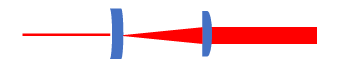
\includegraphics[width=0.5\textwidth]{beam_expansion.png} % 替换为图9实际文件名
  \caption{伽利略式扩束原理图（平凹-平凸透镜组合）}
  \label{fig:beam_expansion}
\end{figure}


\subsubsection{分束与光路的空间规划}
分束环节通过\textbf{无偏振分束棱镜}将扩束后的激光分为光强比近似 $1:1$ 的两束相干光（信号光与参考光）。具体操作要点如下：

\begin{itemize}
  \item \textbf{分束器的空间布局}：将分束棱镜置于平凸透镜出射光路上，使反射支路沿光学平台孔线传输；结合反射镜的紧凑布局，在满足光程设计的同时优化空间利用率。
  \item \textbf{光路准直的迭代优化}：在反射支路上预设光闸 $c$ 和 $d$，采用“远调远、近调近”的迭代方法（同光路准直逻辑），调节反射镜 3 的姿态，使反射光同时穿过光闸 $c$ 与 $d$，确保该支路光轴的直线性与高度一致性。
\end{itemize}

\begin{figure}[htbp]
  \centering
  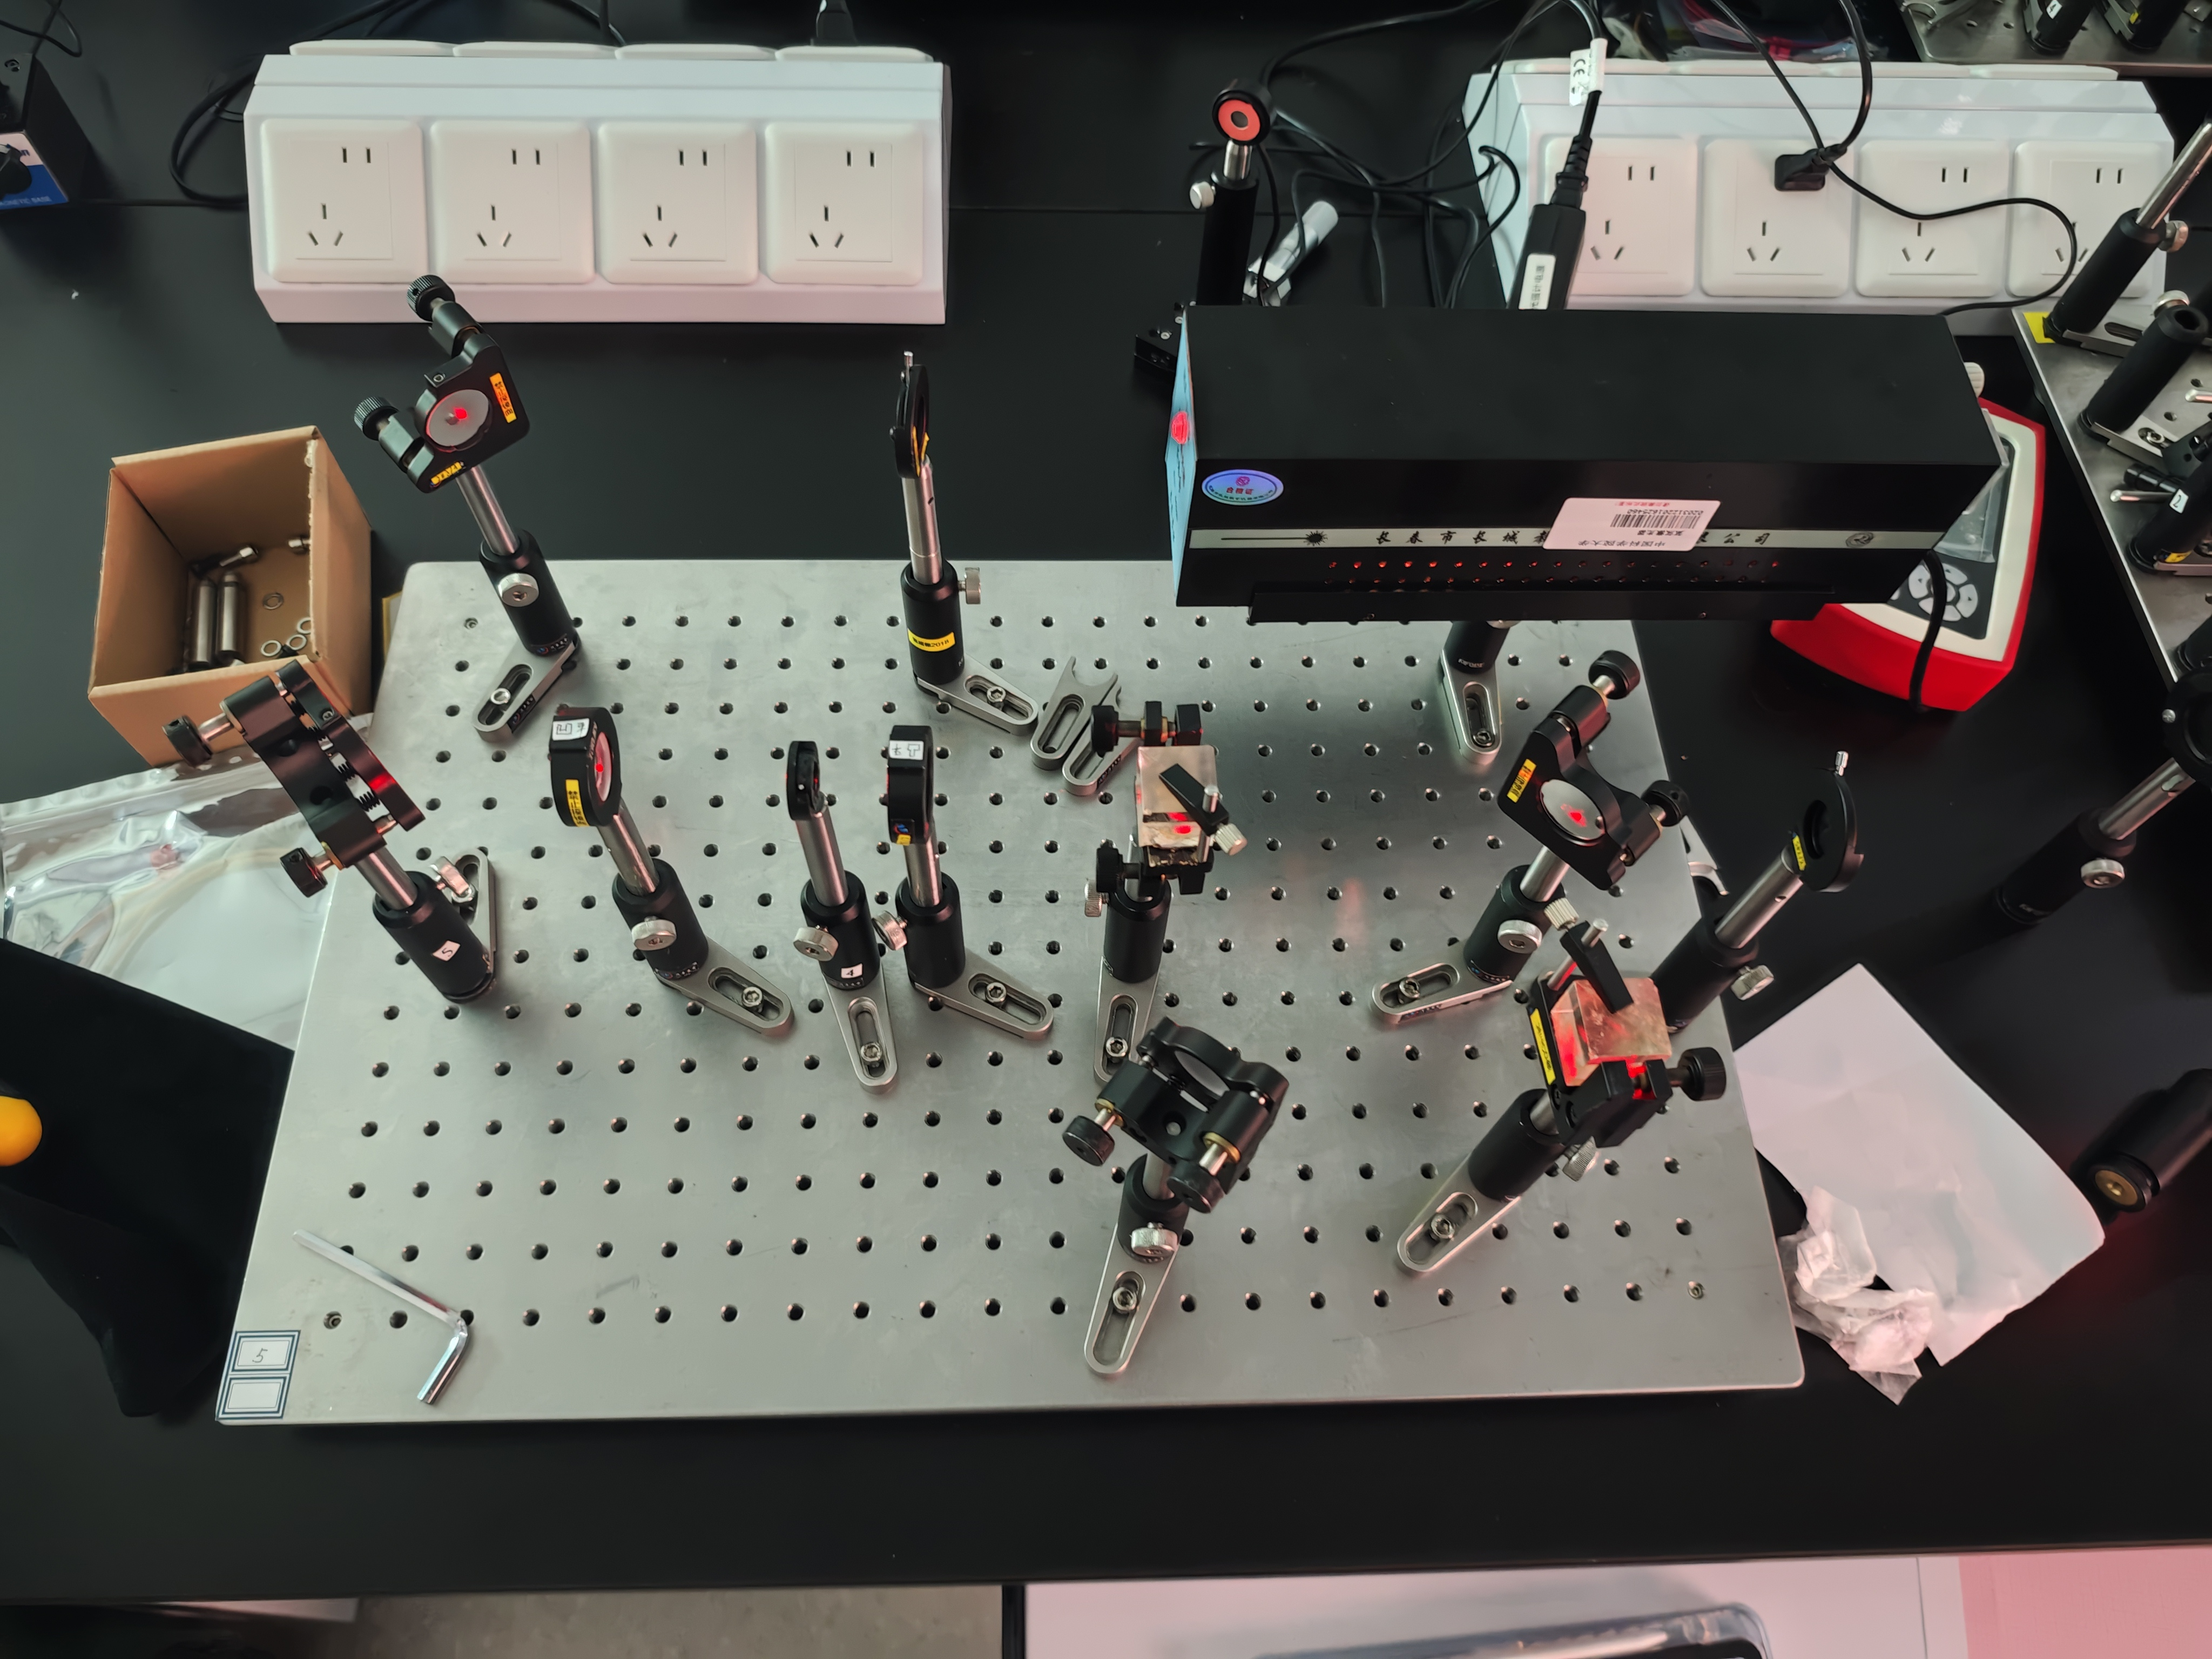
\includegraphics[width=0.6\textwidth]{MZ_beam_splitting.jpg} % 替换为分束光路实际文件名
  \caption{马赫--曾德尔干涉仪分束光路示意图（分束棱镜、反射镜与光闸的协同布局）}
  \label{fig:MZ_beam_splitting}
\end{figure}


\subsubsection{合束系统的调节与光程匹配}
合束的核心目标是使分束后的两路光在\textbf{远场区域精准重合}，以形成稳定的干涉场：

\begin{itemize}
  \item 放置反射镜4，使分束棱镜的透射支路经反射后沿孔线传输；引入合束器（合束 BS），通过远场重合度观测迭代调节反射镜4和合束器的姿态，直至两路光在远场完全叠加，从而保证干涉区域光程差的均匀分布。
\end{itemize}


\subsubsection{干涉条纹的观测与理论分析}

当两路光在远场重合精度满足要求时，白屏上可观测到\textbf{明暗交替的干涉条纹}；遮挡任意一路光，条纹即消失（验证双光束相干机制）。条纹的细节与两路光的重合质量直接相关，理论分析如下：

假设两路相干光存在小夹角 $\alpha$（弧度制）。根据波前干涉原理，等相位面间距与激光波长 $\lambda$ 有关。若相邻两极强点的相位差为 $2\pi$（光程差为 $\lambda$），则条纹间距 $d$ 为：
\begin{equation}\label{eq:fringe_spacing}
d = \frac{\lambda}{2\sin(\alpha/2)} \approx \frac{\lambda}{\alpha},\quad (\alpha \ll 1)
\end{equation}

对于本实验使用的 He--Ne 激光器（$\lambda=632.8\ \text{nm}$），当夹角 $\alpha$ 已知时，可用式\eqref{eq:fringe_spacing}定量计算条纹间距。实验中条纹粗细与间隔会随重合精度变化，反映光程差空间分布的稳定性。

假设两路相干光存在微小夹角\( \alpha \)（弧度制），根据**波前干涉原理**，等相位面间距为激光波长\( \lambda \)。如图\ref{fig:fringe_spacing}所示，相邻干涉极强点（如M和N点）的相位差为\( 2\pi \)，对应光程差为\( \lambda \)，由此推导条纹间距\( d \)的公式：
\begin{equation}
d = \frac{\lambda}{2\sin(\alpha/2)} \approx \frac{\lambda}{\alpha} \quad (\alpha \ll 1,\ \sin\alpha \approx \alpha)
\end{equation}

对于实验采用的He-Ne激光器（\( \lambda = 632.8\ \text{nm} \)），若两路光夹角\( \alpha \)已知，可通过上式定量计算条纹间距。观测中，条纹的粗细、间隔会随两路光的重合精度动态变化，这是光程差空间分布稳定性的直接体现。

\begin{figure}[htbp]
  \centering
  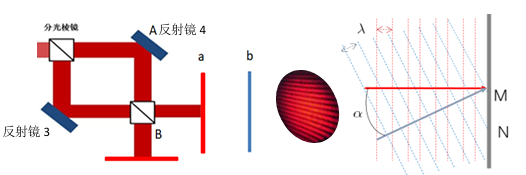
\includegraphics[width=0.6\textwidth]{fringe_spacing.png} % 替换为图10实际文件名
  \caption{干涉条纹间距与两路光夹角的关系（等相位面与条纹形成原理）}
  \label{fig:fringe_spacing}
\end{figure}

\subsubsection{实验结果拍摄}
\begin{figure}[htbp]
  \centering
  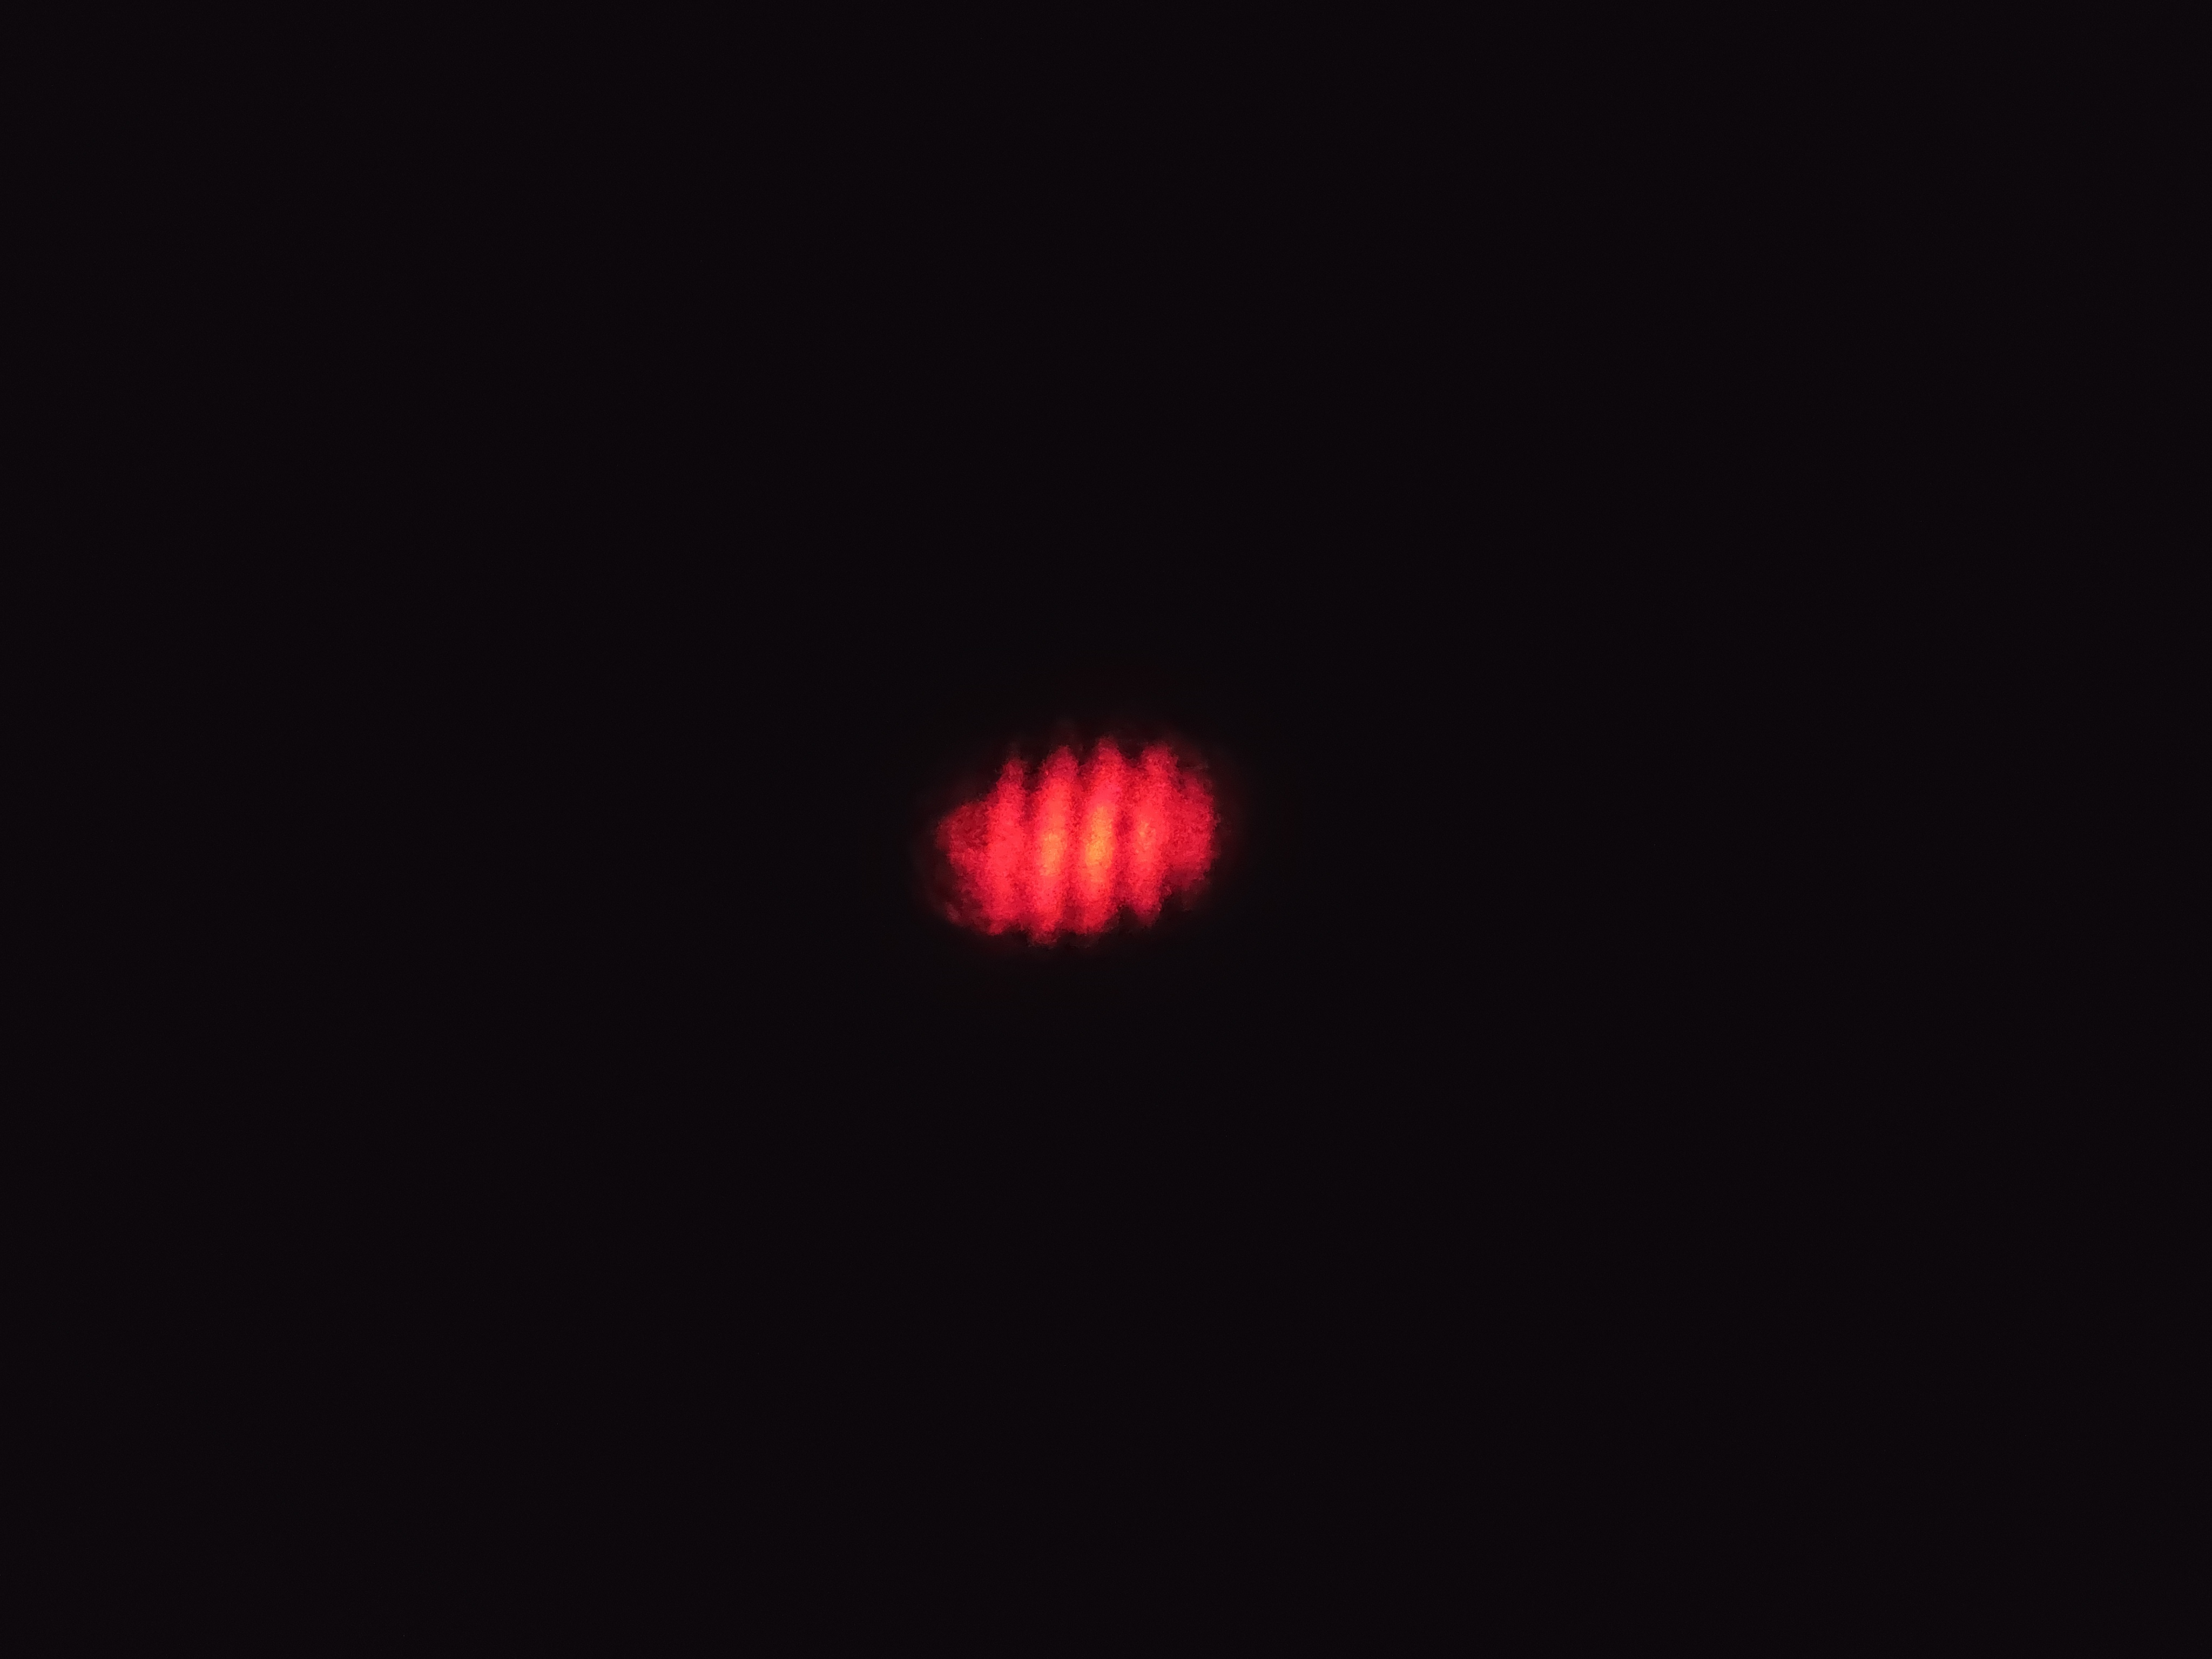
\includegraphics[width=0.6\textwidth]{fig/laserfig.jpg} % 替换为图10实际文件名
  \caption{实验图像：马赫--曾德尔干涉仪干涉条纹实拍图}
  \label{fig:MZ_fringes_photo}
\end{figure}

\subsection{激光偏振态的精密检验与马吕斯定律的实验验证}

激光偏振态的定量检验是偏振光学实验的基础环节。本小节基于\textbf{马吕斯定律}，通过搭建专业光路并开展系统测量，实现对激光偏振


\subsubsection{实验原理与装置架构}
马吕斯定律定量描述了线偏振光经检偏器后的透射光强分布，其核心公式为：
\begin{equation}
I = I_0\cos^2\phi
\end{equation}
其中 $I_0$ 为起偏器出射光强，$\phi$ 为起偏器与检偏器偏振轴的夹角，$I$ 为检偏器出射光强。

实验装置由\textbf{He--Ne 激光器}、光阑、反射镜、起偏器、检偏器、光电池（或功率计）及万用表组成（如图\ref{fig:polarization_test} 所示）。关键设计要求是\textbf{器件共轴性}——所有光学元件的光轴需严格重合，以确保偏振态在传输过程中的一致性和光强测量的准确性。

\begin{itemize}
  \item \textbf{起偏器}：将入射光转换为\textbf{线偏振光}，为实验提供标准偏振态光源；
  \item \textbf{检偏器}：用于分析线偏振光的偏振方向并测量透射光强，其偏振轴角度可调；
  \item \textbf{光电池}：基于光电效应将光强转化为电流信号，通过万用表（mA 或 μA 档）实现电信号的定量读取。
\end{itemize}

\begin{figure}[htbp]
  \centering
  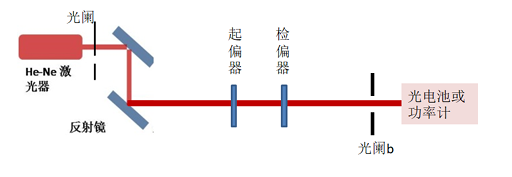
\includegraphics[width=0.7\textwidth]{polarization_test.png} % 请替换为图11实际文件名
  \caption{激光偏振态检验装置示意图（激光器、起偏器、检偏器与光电池的共轴布局）}
  \label{fig:polarization_test}
\end{figure}


\subsubsection{实验操作的精密流程}
本实验的操作需严格遵循“共轴标定 \(\rightarrow\) 偏振轴对准 \(\rightarrow\) 消光验证 \(\rightarrow\) 数据采集”的专业流程，以确保每一步操作的精度与可重复性。

\begin{enumerate}
  \item \textbf{共轴光学系统的精密搭建}
  
  按照“He--Ne 激光器 \(\rightarrow\) 光阑 \(\rightarrow\) 反射镜 \(\rightarrow\) 起偏器 \(\rightarrow\) 检偏器 \(\rightarrow\) 光电池”的顺序，在光学平台上依次安装各个器件。采用“多光阑逐点标定法”对各器件的高度与姿态进行精密调节：确保激光束能够依次、精准地穿过各光阑中心、起偏器与检偏器的通光孔径，并最终完全聚焦于光电池的光敏面中心。此共轴调节的精度直接关系到光强测量的稳定性和准确性，必须反复优化，直至激光束在光路各节点均无偏移。

  \item \textbf{偏振轴初始对准与消光验证}
  
  \begin{itemize}
    \item 旋转检偏器（记为 $P_2$），使光电池输出电流达到最大值，此时起偏器（记为 $P_1$）与 $P_2$ 的偏振轴夹角为 $0^\circ$，标记该位置为初始零点；
    \item 保持 $P_1$ 固定，将 $P_2$ 旋转至 $90^\circ$，此时理论上光强应为 0（消光状态）。若未实现消光，需微调 $P_1$ 至电流最小值并锁定（此步骤为偏振轴正交性的关键标定，后续实验中 $P_1$ 保持不动）。
  \end{itemize}

  实验中需特别注意\textbf{杂散光抑制}：通过光阑遮挡环境光，确保光电池仅接收经起偏器、检偏器的有效偏振光，避免背景光对测量精度的干扰。

  \item \textbf{光强--角度关系的定量测量}
  
  将 $P_2$ 转回 $0^\circ$（光强最大值点），从该位置开始，每旋转 $15^\circ$ 记录一次光电池的电流值 $I$，连续测量至少一个周期（$0^\circ \sim 360^\circ$），以验证 $\cos^2\phi$ 的周期性分布。
\end{enumerate}


\subsubsection{数据处理与物理意义分析}
对实验数据进行专业分析，以验证马吕斯定律并深入理解偏振态特性：

\begin{itemize}
  \item \textbf{归一化与理论拟合}：将各角度下的电流值 $I$ 除以 $0^\circ$ 时的最大电流 $I_{\text{max}}$，得到相对光强 $I/I_{\text{max}}$。将其与理论曲线 $\cos^2\phi$ 进行拟合，通过拟合优度（如 $R^2$）评估实验与理论的符合程度。
  
  \item \textbf{误差来源与优化}：分析实验误差的主要来源，包括：
  \begin{itemize}
    \item 偏振器件的\textbf{消光比}不理想（实际偏振片无法完全消光）；
    \item 光路共轴偏差导致的\textbf{光强泄漏}；
    \item 杂散光与光电池本底噪声的干扰。
  \end{itemize}
  
  针对上述问题，可提出优化方案：选用高消光比偏振片、提升共轴调节精度、增加光阑层数以抑制杂散光等。
\end{itemize}

本实验不仅是马吕斯定律的直接验证，更是理解线偏振光传输、偏振态调控的核心实践，为后续椭圆偏振测量、偏振干涉等复杂实验奠定了技术与理论基础。

\subsection{光纤耦合效率的测量与数值孔径的测量}

光纤耦合效率与数值孔径是表征光纤光学性能的核心参数，前者反映光从自由空间到光纤的功率传输能力，后者描述光纤的集光范围。以下为详细测量方法与步骤。

\subsubsection{光纤耦合效率的精密测量}
光纤耦合效率 \(\eta\) 定义为光纤输出光功率与输入光功率的比值。其精确测量依赖于精密的光路对准与光功率的定量检测，专业步骤如下：

\begin{enumerate}
    \item \textbf{核心器件功能解析}：深入理解光纤跳线、三维/五维调整架、显微物镜系统及光纤支架的操作逻辑，明确多维度精密调整对于实现空间光与光纤模式匹配的关键作用。

    \item \textbf{显微物镜光路准直}：将搭载于五维调整架的显微物镜系统集成至光路中。通过调节其三维调整基座的\textbf{纵向位置、垂直高度及入射角度}，确保激光束经显微物镜聚焦后，其光斑中心能精准穿过远场标靶（如光闸b）的中心孔径，从而建立光纤耦合的基准光轴。

    \item \textbf{调整架光斑中心化标定}：微调五维调整架的平移旋钮（前后、高低），使激光光斑精确位于调整架的机械中心，此举旨在保证光路调节的初始对称性与可重复性。

    \item \textbf{光纤接入与粗对准}：暂时关闭激光源（或使用光闸遮挡），将多模光纤跳线一端接入五维调整架的接口，另一端固定于光纤支架并靠近观察屏。重新开启激光后，通过微调五维调整架的各旋钮，直至在观察屏上观测到明显的光斑，完成粗对准。随后，将光功率计探头紧密贴合光纤输出端面，以确保探测到全部出射光功率。

    \item \textbf{精密对准与功率最大化锁定}：采用迭代优化策略，依次精细微调五维调整架的\textbf{水平角、俯仰角、前后及高低位置}，同时监控光功率计读数。始终沿光功率增强的方向进行调整；若功率下降，则反向或切换至其他维度继续优化，直至功率计读数达到并稳定在最大值。记录此最大输出功率 \(P_{\text{out}}\)。

    \item \textbf{耦合效率计算与光斑模式分析}：移走光纤耦合系统，在显微物镜前测得入射光功率 \(P_{\text{in}}\)。根据公式 \(\eta = \frac{P_{\text{out}}}{P_{\text{in}}} \times 100\%\) 计算耦合效率。同时，定性观测并记录光纤输出光斑的模式特征（如强度分布的均匀性、对称性、有无散斑等）。

    \item \textbf{单模光纤耦合效率的对比测量}：关闭激光，将多模光纤替换为单模光纤。重复步骤4至6，完成单模光纤的耦合效率测量与光斑记录。由于单模光纤芯径极小，对准精度要求更高。

    \item \textbf{多模/单模光纤性能的比较分析}：系统分析两类光纤在耦合效率上的差异，并结合其输出光斑的物理特性（例如，多模光纤的散斑图样 vs. 单模光纤的近高斯分布），从模式数量、模场直径匹配等角度，深入阐释光纤结构对耦合效率的核心影响机制。
\end{enumerate}

\begin{figure}[htbp]
    \centering
    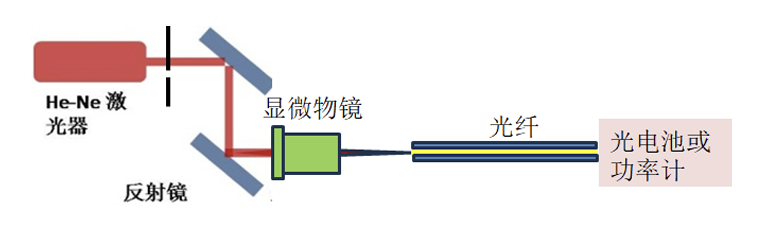
\includegraphics[width=0.8\textwidth]{coupling_test2.png}
    \caption{光纤耦合效率测试光路系统示意图（He-Ne激光器、反射镜、显微物镜、多维调整架上的光纤以及光功率计的级联布局）}
    \label{fig:coupling_efficiency_setup}
\end{figure}

\begin{figure}[htbp]
    \centering
    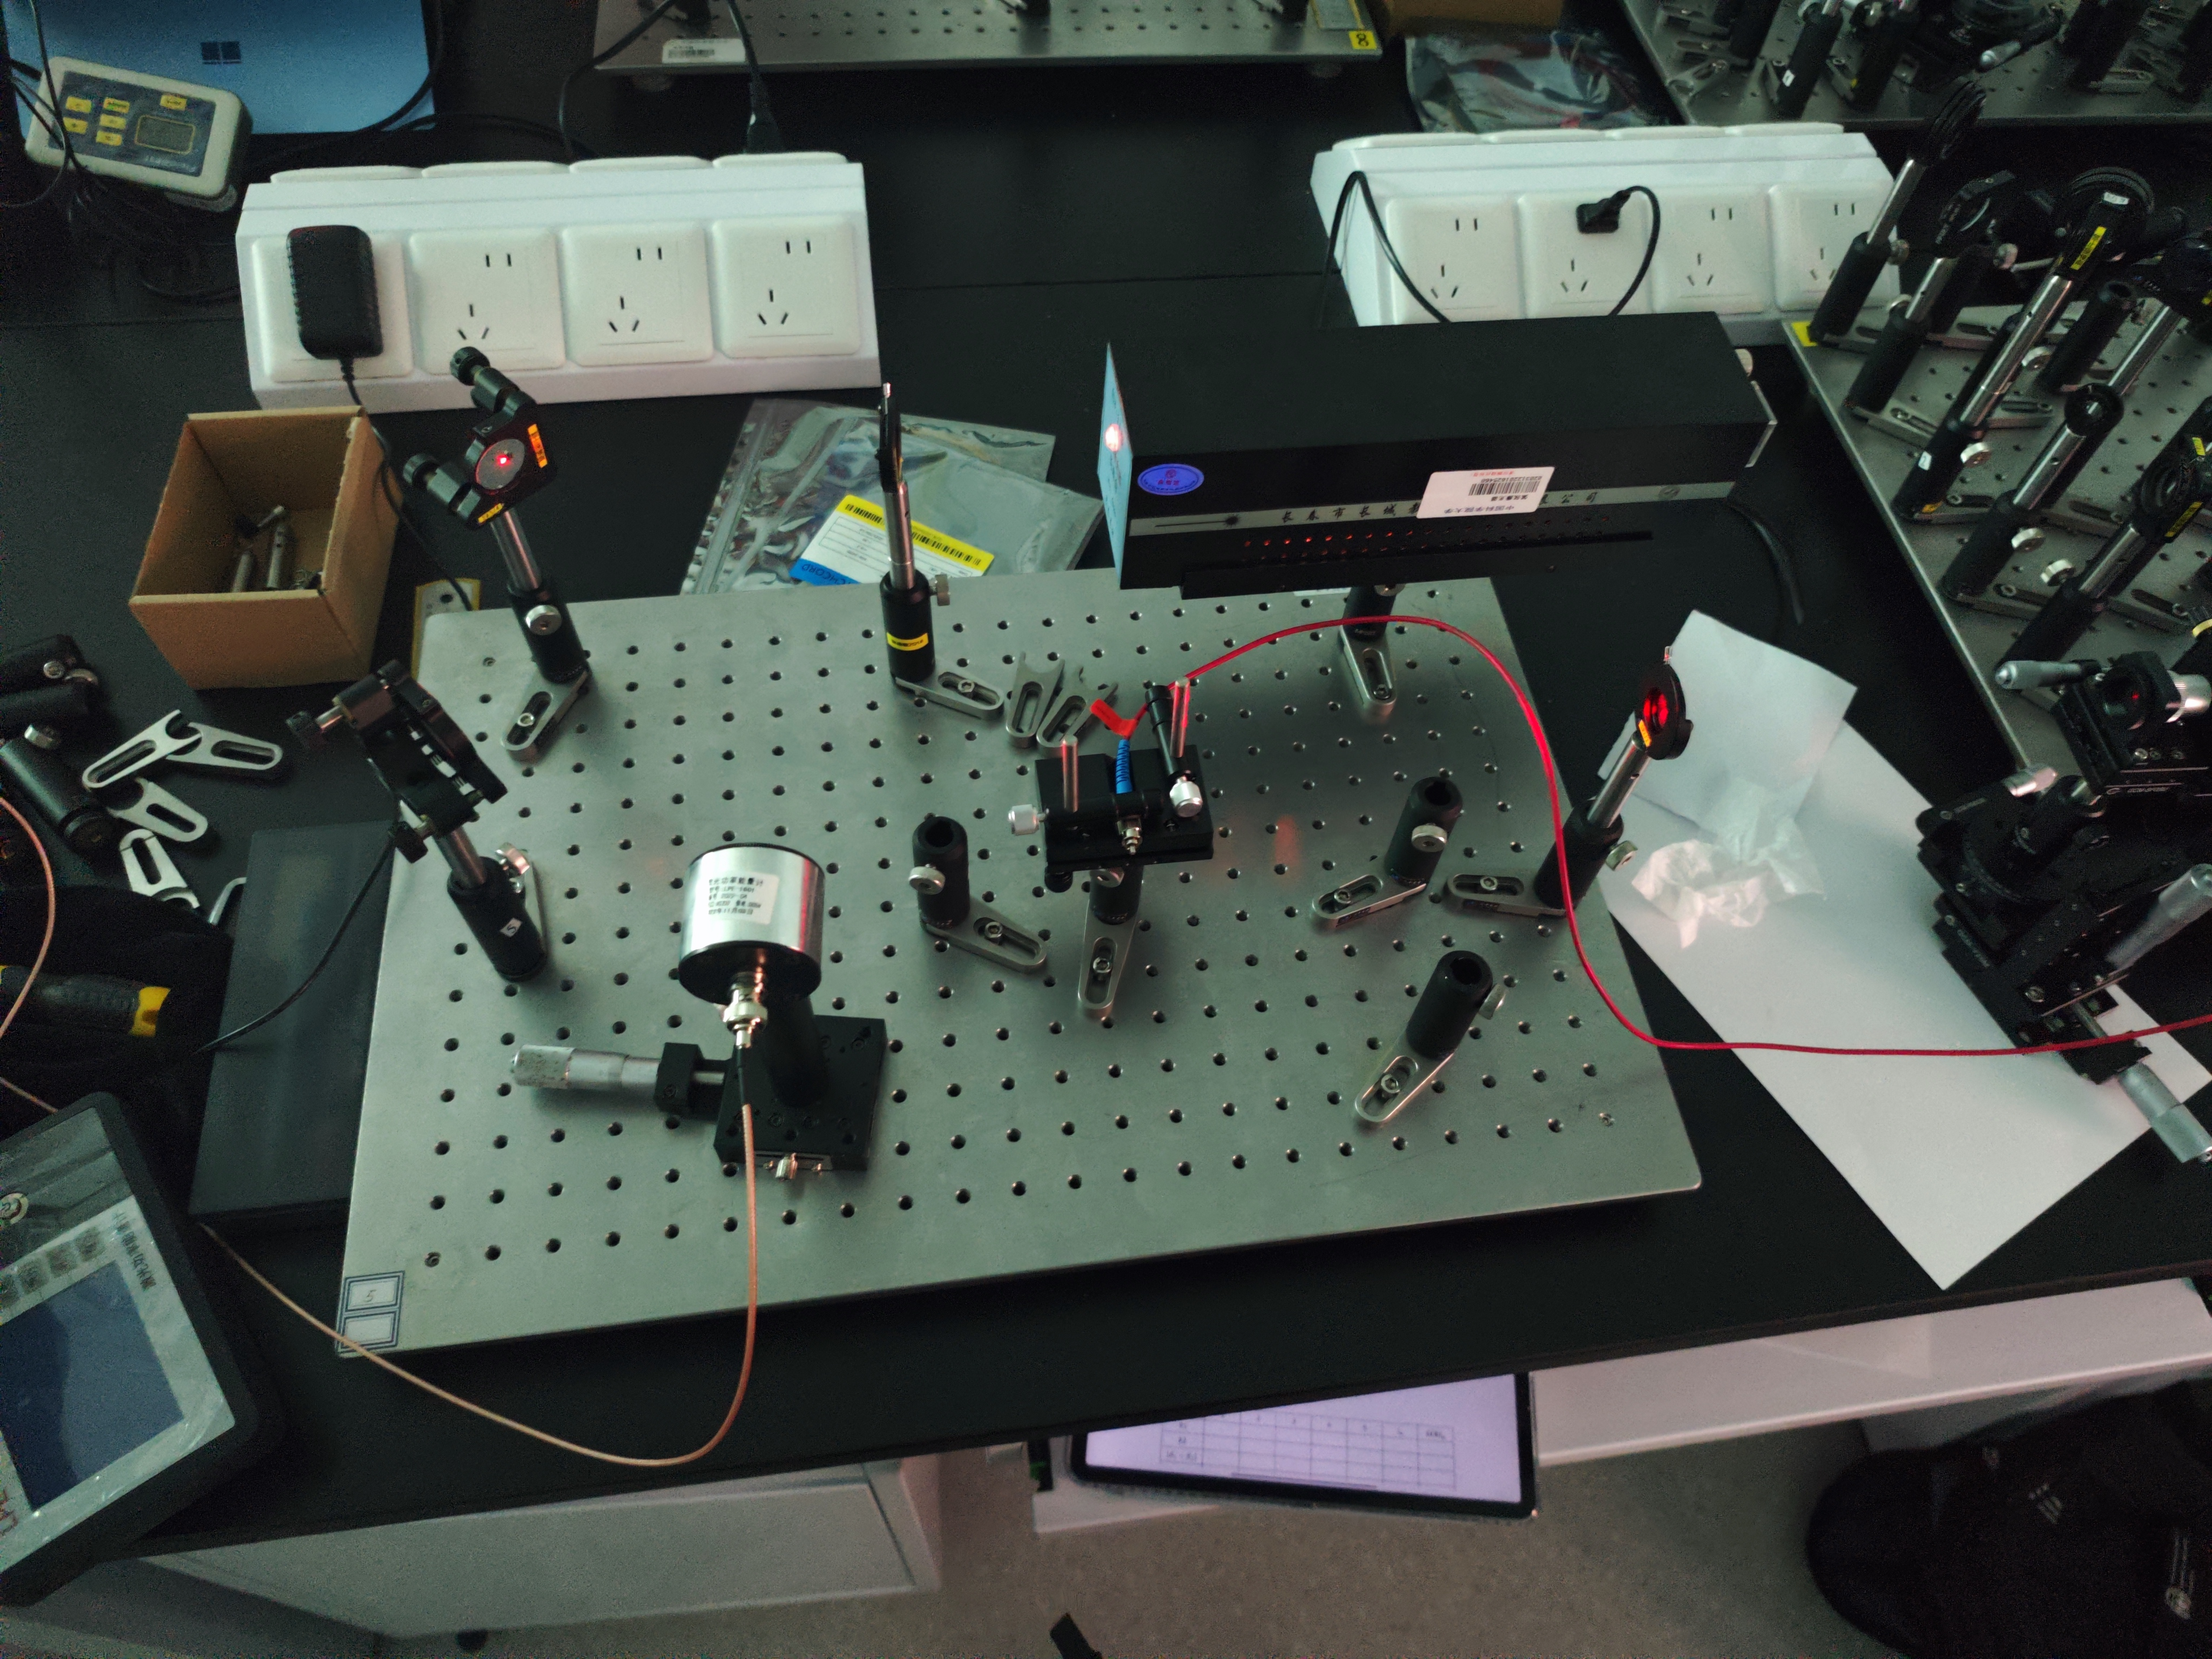
\includegraphics[width=0.8\textwidth]{fig/path 2.jpg}
    \caption{光纤耦合效率测试光路系统示意图（He-Ne激光器、反射镜、显微物镜、多维调整架上的光纤的光路图}
    \label{fig:coupling_efficiency_setup2}
\end{figure}

\subsubsection{光纤数值孔径（NA）的远场法测量}
数值孔径（Numerical Aperture, NA）是衡量光纤集光能力与耦合效率的关键参数。本实验采用\textbf{远场扫描法}，通过测量光纤出射场强度的空间分布来确定其孔径角。

\begin{enumerate}
    \item \textbf{系统校准与稳态建立}：确保激光稳定耦合入单模光纤。将光功率计探头固定于一维精密平移台上，调节探头高度使其光敏面中心与光纤出射光轴严格共轴。
    
    \item \textbf{远场光强分布测量}：
    \begin{itemize}
        \item \textbf{中心峰值定位}：微调平移台位置，搜寻远场光斑中心，记录最大光功率 $P_{\max}$ 及此时平移台读数 $x_c$。
        \item \textbf{有效半径界定}：沿光斑直径方向移动平移台，当光功率下降至约定阈值（通常取 $10\% P_{\max}$ 或 $1/e^2 P_{\max}$）时，记录平移台读数 $x_e$。计算光斑有效半径 $R = |x_e - x_c|$。
    \end{itemize}

    \item \textbf{几何参数标定}：使用直尺或游标卡尺，精确测量光纤输出端面至光功率计探测面的垂直距离 $L$。

    \item \textbf{数值孔径计算}：根据几何光学关系，光纤的最大出射半角（孔径角）$\theta$ 满足 $\tan\theta = R/L$。则数值孔径为：
    \begin{equation}
        \text{NA} = \sin\theta = \sin\left[\arctan\left(\frac{R}{L}\right)\right] \approx \frac{R}{\sqrt{R^2 + L^2}}
    \end{equation}

    \item \textbf{误差控制}：为减小随机误差及光斑非对称性的影响，建议在水平和垂直方向分别测量，或进行多次重复测量取平均值，并计算标准差。
\end{enumerate}
\section{实验数据}


\subsection{数据分析与误差讨论}
\paragraph{数据分析}
为验证马吕斯定律（\(I = I_0 \cos^2\phi\)），我们将实验测得的光强数据进行归一化处理，并与理论值进行比较。取 \(\phi=0^\circ\) 时的光强 \(I_{\text{max}} = 0.566\ \text{mW}\) 作为基准光强 \(I_0\)。归一化后的相对光强 \(I/I_0\) 与理论值 \(\cos^2\phi\) 的对比如下表所示。其中，\(75^\circ\) 时的数据 \(39.7\ \mu\text{W}\) 已转换为 \(0.0397\ \text{mW}\)。

\begin{table}[H]
  \centering
  \caption{马吕斯定律实验数据归一化分析}
  \vspace{0.5em}
  \label{tab:malus_analysis}
  \begin{tabular}{c c c c}
    \toprule
    \textbf{角度 \(\phi\)} & \textbf{测量光强 \(I\) (mW)} & \textbf{理论值 \(\cos^2\phi\)} & \textbf{归一化实验值 \(I/I_0\)} \\
    \midrule
    \(0^\circ\)   & \(0.566\) & \(1.000\) & \(1.000\) \\
    \(15^\circ\)  & \(0.529\) & \(0.933\) & \(0.935\) \\
    \(30^\circ\)  & \(0.426\) & \(0.750\) & \(0.753\) \\
    \(45^\circ\)  & \(0.281\) & \(0.500\) & \(0.497\) \\
    \(60^\circ\)  & \(0.142\) & \(0.250\) & \(0.251\) \\
    \(75^\circ\)  & \(0.0397\) & \(0.067\) & \(0.070\) \\ 
    \(90^\circ\)  & \(0.000\) & \(0.000\) & \(0.000\) \\
    \bottomrule
  \end{tabular}
\end{table}

从 \cref{tab:malus_analysis} 可以看出，归一化后的实验数据与理论预测的 \(\cos^2\phi\) 值高度吻合。在 \(\phi=90^\circ\) 时，光强完全消光，符合理论预期。这表明实验结果很好地验证了马吕斯定律，证明了经起偏器后的激光为线偏振光，且其透射光强与检偏器偏振轴夹角的平方余弦成正比。

\paragraph{误差分析}
尽管实验结果与理论符合得很好，但在精密测量中仍存在不可避免的误差来源，主要可分为以下几类：
\begin{itemize}
    \item \textbf{系统误差}:
    \begin{enumerate}
        \item \textbf{偏振轴对准误差}：起偏器与检偏器刻度盘的 \(0^\circ\) 刻度可能未与偏振轴完全平行，导致测量的角度 \(\phi\) 存在一个系统性的偏移。
        \item \textbf{偏振器件不理想}：实际偏振片的消光比并非无穷大，在偏振轴正交时（\(90^\circ\)）可能仍有微弱的光泄漏，导致测得的最小光强不完全为零。本次实验数据中 \(90^\circ\) 时读数为0，可能是由于功率计精度限制或背景噪声扣除所致。
        \item \textbf{激光功率波动}：He-Ne激光器的输出功率可能随时间有微小漂移，若测量周期较长，会引入系统误差。
        \item \textbf{环境杂散光}：未被完全屏蔽的环境光可能进入光电池，形成一个恒定的背景噪声，对低光强测量（如接近 \(90^\circ\) 时）影响尤为显著。
    \end{enumerate}
    \item \textbf{随机误差}:
    \begin{enumerate}
        \item \textbf{角度读取误差}：在旋转检偏器并读取刻度盘时，存在视差和估读误差。
        \item \textbf{光功率计读数波动}：光电池自身存在热噪声和散粒噪声，导致功率计读数在短时间内有微小起伏。
        \item \textbf{光路准直的微小扰动}：实验过程中的振动或温度变化可能导致光学元件发生微小位移，影响光路共轴性，从而引起光强变化。
    \end{enumerate}
\end{itemize}
总体而言，本次实验操作规范，误差控制在合理范围内，成功验证了马吕斯定律。

\section{预习报告}
\includegraphics[width=0.8\linewidth]{fig/202511102055.pdf}
\end{document}